\documentclass[border=6pt]{standalone}
\usepackage{tikz}
\usetikzlibrary{decorations.pathmorphing, patterns}

\begin{document}
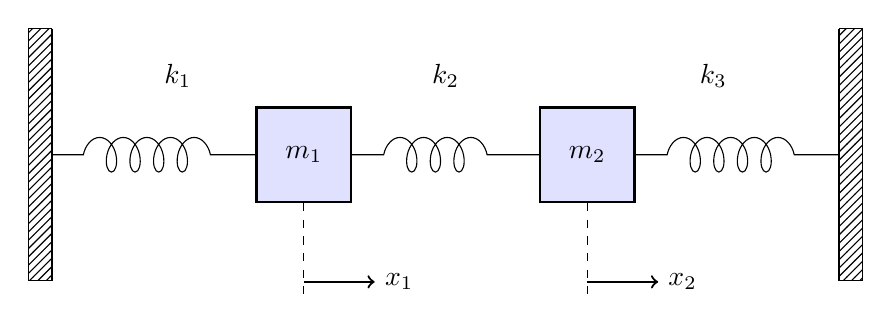
\begin{tikzpicture}[
  spring/.style={
    decorate,
    decoration={coil, aspect=0.6, segment length=3mm, amplitude=2.2mm,
                pre length=4mm, post length=4mm}
  },
  wall/.style={
    pattern=north east lines, draw
  },
  mass/.style={
    draw, thick, fill=blue!12, minimum width=12mm, minimum height=12mm
  }
]

% geometry
\def\ymid{0}          % vertical center line
\def\wallh{1.6}       % wall half-height

% left wall
\fill[wall] (-0.3,-\wallh) rectangle (0,\wallh);
\draw[thick] (0,-\wallh) -- (0,\wallh);
% right wall
\fill[wall] (10,-\wallh) rectangle (10.3,\wallh);
\draw[thick] (10,-\wallh) -- (10,\wallh);

% masses
\node[mass] (m1) at (3.2,\ymid) {$m_1$};
\node[mass] (m2) at (6.8,\ymid) {$m_2$};

% springs (left wall -> m1 -> m2 -> right wall)
\draw[spring] (0,\ymid) -- (m1.west);
\draw[spring] (m1.east) -- (m2.west);
\draw[spring] (m2.east) -- (10,\ymid);

% spring labels
\node at (1.6,1.0) {$k_1$};
\node at (5.0,1.0) {$k_2$};
\node at (8.4,1.0) {$k_3$};

% displacement coordinates
\draw[->, thick] (m1.south) ++(0,-1.0) -- ++(0.9,0) node[right] {$x_1$};
\draw[->, thick] (m2.south) ++(0,-1.0) -- ++(0.9,0) node[right] {$x_2$};
\draw[dashed] (m1.south) -- ++(0,-1.2);
\draw[dashed] (m2.south) -- ++(0,-1.2);

\end{tikzpicture}
\end{document}
